\ifx\wholebook\relax\else
\input{../Common.tex}
\input{../macroes.tex}
\begin{document}
\fi

\chapter{Coordinates, Points and Absolute Moves}\label{ch:absoluteLocation}\label{cha:absoluteLocation}

%\hrule\vskip 1ex
%\begin{minipage}[t]{\linewidth}
%\hfil \includegraphics[width=0.9\linewidth]{picasName}\hfil
%\end{minipage}
%\vskip 1ex\hrule\vskip 5ex


Up to now the messages sent to a robot to move it were relative to its current position. Indeed, the expression \ct{pica\ go:\ 100} means that you ask a robot to go forward 100 pixels from its current position in its current direction. Such a move is said to be \emph{relative} because the position reached by the robot at the end of the move depends on its initial position. This kind of move is very powerful but sometimes you would like to be able to say to a robot to move to a specific location on the screen such as the middle of the screen, that is make a robot move in a \strong{absolute} manner. For this purpose we need a coordinate system, \ie a way to represent a specific location on the screen. You use a coordinate system when you are looking for a street on a map. The map listing indicates that a given street is located in a square identified by one letter and a number or two letters or two numbers. The same applies to computer screen. You can refer to a location given a point \ie\ a pair of numbers. Therefore in this chapter I start to present points and coordinates, then I present new robot behavior and some experiments. This will help us to explore new problems in the future such as using robots to simulate animal behavior.

\begin{figure}
\begin{center}
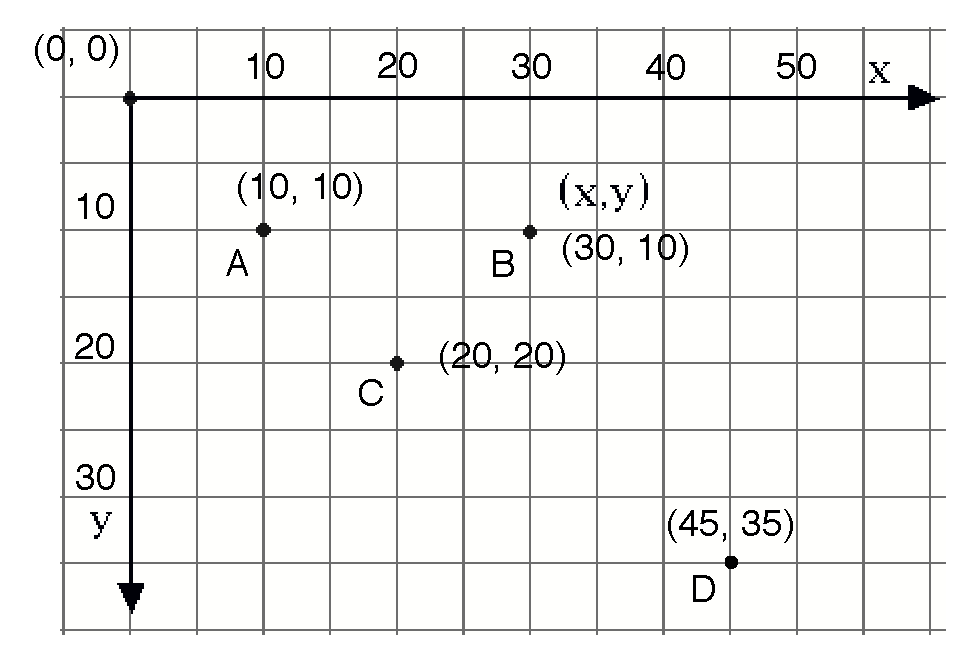
\includegraphics[width=8cm]{PointsReperes}
\caption{A point represents a location in a two dimension area. A point has an x or horizontal coordinates and a y or vertical coordinates.\label{fig:PointsRepere}}
\end{center}
\end{figure}

\section{Points}
Since everything in \st is an object, locations on the screen are {\em also} described by objects called \emph{points}. Points are created by the class \ct{Point} and their behavior is close to the mathematical one.  In two dimensions a point is composed of two coordinates: $x$ (the point horizontal coordinates) and $y$ (the point vertical coordinates).
A point is created by sending the message \ct{@}\index{@} sent to a number. For example, the point D of Figure~\ref{fig:PointsRepere} is created by the expression \ct{45@35}. A's x is \ct{45} and y is \ct{35}.  

\cadre{\ct{200@400} is a point whose x is 200 and y 400.}

The following script~\ref{scr:pointope} presents how to access point constituents. 

\begin{scriptwithtitle}{Point element access}\label{scr:pointope}
| point1 |
point1 := 45@35.
point1 x
-> 45
point1 y 
-> 35
\end{scriptwithtitle}

It is worth to pay attention that the coordinate system in \st is not completely the same that the mathematical one. Figure~\ref{fig:PointsRepere} shows that contrary to the mathematical model, the y axis goes positive from the top to the bottom of the screen while the x axis goes increasing from left to right. We say that in \sq the origin of the coordinate system is the top left corner of the screen. In a mathematical system the y axis goes from the bottom to the top. Thus, the point \ct{45@35} is located 45 pixels from the left side  and 35 pixels from the top of the screen. 

\cadre{The \st coordinate system has its origin (0,0) on the top left corner of the screen and y axis goes positive from top to bottom.}

All kinds of mathematical operations are available on the points. In this chapter we will only present some of operations that we shall use in the future.  \st goes a step further that proposing the basic mathematical operation. For example, we can multiply a point by a value to get a point whose values is the previous ones but multiplied by this value \ct{(100@200) * 3}, or use common mathematical operation such as addition, substraction on points themselves. Note that the binary operations such as -, *, + creates new points.  The script~\ref{scr:pointmultiple} shows different operations.


\begin{scriptwithtitle}{Point manipulation}\label{scr:pointmultiple}
| point1 point2 point3 |
point1 := 200@400.
point2 := point1 * 2
point2 
\pr 400@800
point2 x
\pr 400
point2 y
\pr 800
point3 := (50@60) + point1.
point3 x
\pr 250
point3 y
\pr 460
point1 + 200      "200 is considered as the point 200@200"
\pr 400@400
\end{scriptwithtitle}


\section{Using Grids}
To help you to understand points, you can have a look at the information displayed in the balloon that pops up when you let the mouse over your robots. You can also use a grid. Indeed, \sq can draw a grid on the background of the screen. To get the grids, bring the \menu{world} menu, select \menu{playfield options...}, and the menu items \menu{use standard texture} or \menu{make graph paper...}. Choosing the last one lets you define the size and the color of the grid. 

As shown by  \scrref{scr:grid}, you can also program the grid using  the following methods: \index{drawGrids}\ct{drawGrids} and \index{undrawGrids}\ct{undrawGrids}, to draw and undraw the grids, \index{gridColor:}\ct{gridColor: aColor} to change the color of the grids, \index{gridSize: anInteger}\ct{gridSize: anInteger} to specify the size of the grid, \index{gridWorldColor:} \ct{gridWorldColor: aColor} to change the color of the world when the grid is drawn, and \index{worldColor: aColor }\ct{worldColor: aColor} to change the color of the world. You can also get the size of the grid using the method \ct{gridSize}.

\begin{scriptwithtitle}{Setting the grids.}\label{scr:grid}
| env | 
env := BotEnvironment default.
env gridSize: 25.
env gridWorldColor: Color paleBlue.
env gridColor: Color blue.
env drawGrids
\end{scriptwithtitle}

\begin{figure}
\begin{center}
\includegraphics[width=6cm]{spiderWithGrids}
\end{center}
\caption{Grids of 25 pixels. \label{fig:spiderWithGrids}}
\end{figure}

Using the \menu{World} menu you can change the size of the screen. 
To go on full screen, bring the world menu, select \menu{appearance...} and then the full screen on or off menu item. You can also use the following methods \index{fullScreenOff} \ct{fullScreenOff} \index{fullScreenOn} \ct{fullScreenOn} as shown in~\tscrref{scr:screenSize}.

\begin{scriptwithtitle}{Setting the screen size}\label{scr:screenSize}
BotEnvironment default fullScreenOn
\end{scriptwithtitle}



\section{Source of Errors with Points}

The way points are created may lead to some errors as shown by the first line of the \scrref{scr:pointprob}. \ct{50@60 + 200@400} returns \ct{aB3dVector} instead of a point representing the sum of the two points. The problem is that when a point, and not an integer, receives the message \ct{@}, it returns another kind of point that does not interest us.  Therefore we should pay attention to the way the messages are sent as explained below.

\begin{scriptwithtitle}{Possible error with points}\label{scr:pointprob}
50@60 + 200@400
->  a B3DVector3(250.0 260.0 400.0)
"returns a 3D vector but not a point"

(50@60) + (200@400)
-> 250@460
\end{scriptwithtitle}

\largecadre{To avoid trouble with points, surround them with parenthesis when they are involved in complex operation.}

As explained in \charef{ch:Evaluating}, you should know how messages are executed and in particular
\begin{itemize}
\item that parentheses \ct{()} are evaluated first,  
\item that {\em unary} messages are executed before {\em binary} ones and that \emph{binary} messages are executed before {\em keywords-based} ones and 
\item that  messages of the same kind are evaluated from left to right. 
\end{itemize}

Here the method \ct{@} is just a binary method like any other and it has the same priority that binary methods such as \ct{+}, \ct{*}, or \ct{//}. Therefore the expression \ct{50@60 + 200@400} is executed as it would have been typed as follows \ct{(((50@60) + 200) @ 400)}. The message \ct{@} will be sent to a point and not an integer. Let us look at what happens in the first line of the script~\ref{scr:pointprob} which does not correctly returns the point \ct{250@460} as we expected. The script~\ref{scr:understanding} shows how the messages are executed. 

\begin{scriptwithtitle}{Decomposing \ct{50@60 + 200@400}}\label{scr:understanding}
50@60 + 200@400 {\rmfamily is equivalent to }(((50@60) + 200) @ 400)
{\rmfamily
{\textbf Step 1}
   \ct{@} is sent to \ct{50} with the argument \ct{60}, it returns the point \ct{50@60}. 
{\textbf Step 2}
   \ct{+} is sent to the point \ct{50@60} with the argument \ct{200}, it returns
   \ct{250@260} because when a number is passed as an argument it is 
   considered as the point having the same value for x and y. 
   Here \ct{200@200}. 
{\textbf Step 3} 
   \ct{@} is sent to \ct{250@260} with \ct{400} as argument, the object
   \ct{B3DVector3(250.0 260.0 400.0)} is returned.}
\end{scriptwithtitle}

Now when we simply put parenthesis around the points we obtain a point that is the sum of the two others as explained by the script~\ref{scr:understanding2}.

\begin{scriptwithtitle}{Decomposing \ct{(50@60) + (200@400)}}\label{scr:understanding2}
(50@60) + (200@400)
{\rmfamily
{\textbf Step 1} 
   Parenthesis are evaluated first.
{\textbf Step 1.1} 
  \ct{@} is sent to \ct{50} with \ct{60} as argument and returns a point.
{\textbf Step 1.2} 
  \ct{@} is sent to \ct{200} with \ct{400} as argument and returns a point.
{\textbf Step 2} 
   \ct{+} is sent to \ct{50@60} with argument \ct{200@400} and 
    returns the new point \ct{250@460}.}
\end{scriptwithtitle}

In summary we suggest you to put parenthesis around points when you are doing point manipulation.

\section{Absolute Moves}
Now that we can specify a location on the screen, we can ask a robot to go directly to a given location. For this task two methods \ct{goTo: aPoint}\index{goTo:} and  \ct{jumpTo: aPoint}\index{jumpTo:} exist. 
\begin{itemize}
\item Sending the message \ct{goTo: aPoint} to a robot, asks it to go to the location represented by the point. 
\item Sending the message \ct{jumpTo: aPoint} to a robot asks it to jump to the location
 represented by the point.
\end{itemize}

Note that the message \ct{jump:} and \ct{jumpTo:} do not leave a trace, while \ct{go:}and \ct{goTo:} do. Let us practice now. Try to guess what script~\ref{scr:moveToPoint} does.
As another experience, try to guess the size of your screen by positioning a robot as close as possible to the bottom right corner. 

\begin{scriptwithtitle}{Going directly at a location and jumping.}\label{scr:moveToPoint}
| pica  |
pica := Bot new.
pica goTo: 200@400.
pica jumpTo: 300@400.
pica go: 1.
pica jumpTo: 400@400.
pica goTo: 450@400
\end{scriptwithtitle}

The following section will stress the difference the methods \ct{go: aDistance} and \ct{goTo: aPoint}, and \ct{jump: aDistance} and \ct{jumpTo: aPoint}.


\section{Relative vs. Absolute Motions}
Now we shall look at the difference between the methods  \ct{go: aDistance} and \ct{goTo: aPoint}. The method \ct{go:} asks a robot to move of a given distance \emph{along its current direction}. Thus, the robot position depends on its current location and of its current direction. Script~\ref{scr:moveToPoint} illustrates this.

\begin{scriptfig}{dualMotion}{Parallel motion}
\label{scr:dualMotion}
| pica marge |
pica := Bot new.
marge := Bot new.
marge lookLikeTriangle.
pica lookLikeCircle.
marge color: Color red.
marge penSize: 3.
marge north.
marge jump: 50.
marge east.
\bold{pica go: 200.
marge go: 200.}
\end{scriptfig}

As you can see, the two robots are moving along parallel lines and
do not end up in the same location, even though the same message
\ct{go:\ 200} was issued to them at the end of the script.

On the contrary, the method \ct{goTo: aPoint} asks a robot to place itself
to a fixed location \emph{regardless} of its position and direction
before the move. This is illustrated by
\scrref{scr:convergentMotion}.

\begin{scriptfig}{convergentMotion}{Convergent motion}
\label{scr:convergentMotion}
| pica marge |
pica := Bot new.
marge := Bot new.
marge lookLikeTriangle.
pica lookLikeCircle.
marge color: Color red.
marge penSize: 3.
marge north.
marge jump: 50.
marge east.
pica goTo: World center - 100.
marge goTo: World center - 100. 
\end{scriptfig}

In this case, the two robots end up at the same location. One says that the method \go produces a \emph{relative} motion, whereas the method \ct{goTo:} produces an \emph{absolute} motion. In the previous script we use the expression \ct{World center - 100} so that you get exactly the same picture as the one we show even if you computer has a different resolution than the one used to 
write this book. 

Finally note that the methods \go and \ct{goTo:} do not change the direction of the robot. This is illustrated by \scrref{scr:combinedMove}. In this script we ask a robot to move forward 100 pixels from its current position, then  asks it to go directly to a position that is located at 100, -100 from the center of the screen, and then move forward again 100.

\begin{scriptfig}{zebra}{Combining absolute and relative motions}
\label{scr:combinedMove}
| pica |
pica := Bot new.
pica lookLikeCircle.
pica north.
pica go: 100.
pica goTo: (World center - (100@-100)).
pica go: 100.
\end{scriptfig}


\section{Some Experiments}
Now we propose you some experiences you get more familiar with the concepts presented.  As you can see, the robot does not change its direction when it is transported to a given location using \ct{goTo:}

\begin{exonofig}\label{exo:rectangle}
Using the methods \ct{goTo:} and \ct{jumpTo:} define a method \ct{rectangleTopLeft: point1 bottomRight: point2} that draws a rectangle. For example, 
\ct{pica rectangleTopLeft: 200@500 bottomRight: 350@700}.
\end{exonofig}

\comment{
\begin{scriptwithtitle}{Absolute Rectangle}
| pica point1 point2|
pica := Bot new.
point1 := 350@500.
point2 := 200@600.
pica jumpTo: point1.
pica goTo: point1 x @ point2 y.
pica goTo: point2.
pica goTo: point2 x @ point1 y.
pica goTo: point1
\end{scriptwithtitle}
}

\begin{exonofig}\label{exo:rectangle2}
Define another method \ct{rectangleOrigin: point1 extent: point2} that the second point does not represent anymore the opposite corner but the size of the rectangle. For example \ct{pica rectangleOrigin: 200@600 extent: 350@500} we will have a rectangle starting at location \ct{200@600} and having a height of 350 and width of 500. \end{exonofig}

\section{Translations}
When we add the same amount to all the points of a shape, we obtain the same shape but in another position. This operation is called a translation in mathematics. As shown in Figure~\ref{fig:translatedTriangleExplained} the amount that we add to the points of the original shape can be different for the x and y axis, therefore it can be represented as a point and the translation is simply expressed as the sum between a vertice and a point representing the translation. A vertice of the new figure is equal to the sum of a point of the translated figure and the translation point. 
In Figure~\ref{fig:translatedTriangleExplained} the vertice (x1, y1) is translated by adding
the point translation and the result is a point whose $xnew = x1 + translation\ x$, and $ynew = y1 + translation\ y$. For example,  the point \ct{200@300} translated by the translation point \ct{50@75} is \ct{250@375}. 

\begin{figure}
\begin{center}
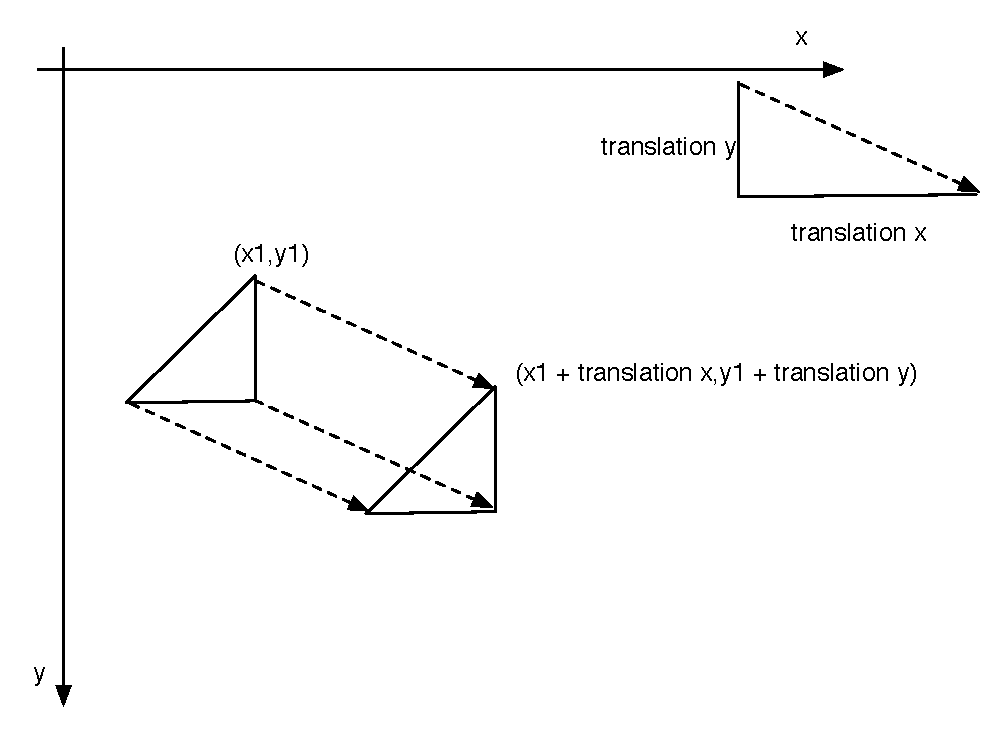
\includegraphics[width=6cm]{translatedTriangleExplained}
\end{center}
\caption{Translating a shape requires to add to each point of the shape the same amount for each axis. \label{fig:translatedTriangleExplained}}
\end{figure}


\paragraph{Triangle.}
Define a method named \ct{triangleAt: point1 point2: point2 point3: point3} which draws a triangle between the points given as arguments. \Tscrref{scr:triangleUse} illustrates how to use such a method.

\begin{scriptfig}{triangleByPoints}{Using \ct{triangleAt:point2:point3:}}\label{scr:triangleUse}
| pica |
pica := Bot new.
pica  
   triangleAt: 200@300 
   point2: 200@250 
   point3: 150@300 
\end{scriptfig}


\paragraph{Translating Triangles}
Now we can draw several triangles by simply translating the first one. In script~\ref{scr:translated}, we define three translations and draw the corresponding triangles. 

\begin{scriptfig}{translatedTriangles}{Using \ct{triangleAt:point2:point3:}}\label{scr:translated}
| pica  point1 point2 point3 t1 t2 t3 |
point1 := 200@300.
point2 := 200@250.
point3 := 150@300.
t1 := -50@-50.
t2 := 90@150.
t3 := 150@90.
pica := Bot new.
pica beInvisible.
pica triangleAt: point1 point2: point2 point3: point3.
pica triangleAt: point1 + t1 point2: point2 + t1 
        point3: point3 + t1.
pica triangleAt: point1 + t2 point2: point2 + t2 
        point3: point3 + t2.
pica triangleAt: point1 + t3 point2: point2 + t3 
        point3: point3 + t3.
\end{scriptfig}

We could also have define another method \ct{triangleAt:point2:point3:translation:} that performs the translation instead of having to do ourselves the point addition. Such a solution is safer since we cannot apply different translations to different points of the same triangle and therefore we suggest you to implement it. 

\paragraph{Flying Geese.}
One can repeat the translation operation to obtain repeating patterns. The script~\scrref{scr:newflyinggeese} generates the pattern called \emph{flying
geese} in patchwork. Note that  we chose the amount of translation so that the next triangle is in diagonal.

\begin{scriptfig}{flyingGeese}{Flying Geese}\label{scr:newflyinggeese}
| pica translation point1 point2 point3 |
point1 := 200@300.
point2 := 200@250.
point3 := 150@300.
translation := 25@25.
pica := Bot new.
10 timesRepeat: 
        [ pica triangleAt: point1 point2: point2 point3: point3.
        point1 := point1 + translation.
        point2 := point2 + translation.
        point3 := point3 + translation].
\end{scriptfig}


Script~\ref{scr:newflyinggeese2} shows how we can write the translation in a more concise way using the fact that we can multiply points too. 

\begin{scriptwithtitle}{Flying Geese}\label{scr:newflyinggeese2}
| pica  times |
pica := Bot new.
times := 1.
10 timesRepeat: 
        [ pica triangleAt: 200@300 
                    point2: 200@250 
                    point3: 150@300 translation: (25@25) * times.
        times := times + 1].
\end{scriptwithtitle}


\begin{exofig}{triangleByDelta}
As a variation of the same problem, define another method named \ct{triangleAt: aPoint delta1: aPoint1 delta2: aPoint2} that starts to draw a triangle at the point \ct{aPoint} then uses the two following arguments as differences between points by reference  to the first point.
So that \ct{t triangleAt: 200@300 delta1: 0@-50 delta2: -50@50} draws the same triangle as: 
\ct{t triangleAt: 200@300 point2: 200@250 point3: 150@300}
\end{exofig}



\section{Absolute Moves at Work}
Now you may wonder why does one need points? So far, all drawings did not require points. In fact executing most drawings using points would have been quite difficult. Imagine how difficult can be  to draw a pentagon only using the \ct{goTo:} message. 
Still absolute positions are useful. The following illustrates such an example. 
We will use a point to keep track of the robot position at a given moment during the execution of a complex drawing. Then we will used this position to continue our drawing from this place. 

The first example is based on the \scrref{scr:letterA} of
chapter \ref{ch:robotMen} in which we were drawing the letter A. At the end of Section \ref{sec:abcDraw} we noted that the bottom
half of the left bar of the "A" is drawn twice by the 
\scrref{scr:letterA}. We considered that it was not
that big a problem.  Our solution is to use a point to store the location of the robot, location to which the drawing requires to come back later.

Let us modify the \scrref{scr:letterA} as shown in the script~\ref{scr:relativeA} to get the possibility to draw an A letter in a relative way.  

\begin{scriptwithtitle}{An A relative}\label{scr:relativeA}
| pica |
pica := Bot new.
pica turnLeft: 90.
pica go: 100.
pica turnRight: 90.
pica go: 100.
pica turnRight: 90.
pica go: 100.
pica turnRight: 180.
pica go: 50.
pica turnLeft: 90.
pica go: 100
\end{scriptwithtitle}

Now we modify this script as shown in the script~\ref{scr:absoluteA}. 

\begin{scriptfig}{turtleMLetterA}{The letter "A" is any direction}\label{scr:absoluteA}
| pica \bold{barPoint} |
pica := Bot new.
pica turnLeft: 90.
pica go: 40.
\bold{barPoint := pica center.}
pica go: 60.
pica turnRight: 90.
pica go: 100.
pica turnRight: 90.
pica go: 100.
\bold{pica jumpTo: barPoint.}
pica turnLeft: 90.
pica go: 100\end{scriptfig}

In \scrref{scr:absoluteA}, the first vertical bar of the "A"
is drawn in two steps first 40 then 60 pixels. Between the steps, the absolute location of the robot is obtained using the method \ct{center}\index{center}. This is the location where the bar of the "A" should be drawn. The result of that method is stored in the variable \ct{barPoint}. After the last vertical bar is drawn, the robot goes back to the location of the bar using the method \ct{goTo:\ barPoint}. From this point on, the bar is drawn.


By the way you can verify that the letter "A" is indeed drawn correctly in any direction by adding a command \ct{turnLeft:} or
\ct{turnRight:} after the creation of the robot. 


 
\begin{exofig}{chAbsArrow}\label{exo:arrows}
Using the same technique, define a script that generates 8 arrows shooting from the robot origin in 8 different directions as shown in the neighboring figure. 
Hint: Define first a method called \ct{arrow: aPoint} that draws an arrow pointing in the current 
direction starting at the given point. Then use a additional variable to remember the origin of the arrow.
Once you get done you strongly recommend you to redo the same experiment using the method \go and \jump. This way you will really touch the difference between the two ways of expressing 
the same problem.
\end{exofig}

\section{Loops and Translations}
Before reading the following, try to define the script that draws Figure~\ref{scr:flyingGeeseQuit}.

Now we explain how we can produce the drawing shown in Figure~\ref{scr:flyingGeeseQuit}. 

Points define a lot of useful methods from which we explain ones  we use in the script~\ref{scr:flyingGeeseQuit}: \ct{negated} and \ct{setX:setY:}.
\begin{itemize}
\item 
The method \ct{negated} sent to a point returns a point whose
x and y are negated value of the receiving
point. Thus, the point \ct{(200@400)\
negated} is the point \ct{-200@-400}. Note that the
parentheses are necessary. Indeed, \ct{negated} is also a
method understood by numbers. Thus, the expression
\ct{200@400\ negated} yields the point \ct{200@-400}
because the method \ct{negated} being an unary method 
is executed before the method \ct{@} by the
number \ct{400}. In \tscrref{scr:flyingGeeseQuit} we use this
method to produce a translation in the opposite direction.

\item The method \ct{setX:setY:} changes the constituents of a point.
Thus, if \ct{point} is any point, after executing the expression
\ct{point\ setX: 200\ setY: 400}, the point has for x value \ct{200} and for y value \ct{400}. 
\end{itemize}

\begin{scriptfig}{flyingGeeseQuit}{Flying geese cover quilt}
\label{scr:flyingGeeseQuit}
| pica point1 move shift|
point1 := 200@300.
move := 25@0.
shift := -25@50.
pica := Bot new.
5 timesRepeat: 
     [ 10 timesRepeat: 
          [ pica 
               triangleAt: point1 
               delta1: 25@-25 
               delta2: -25@-25.
           point1 := point1 + move ].
     point1 := point1 + shift.
     move := move negated.
     shift setX: shift x negated setY: shift y ].
\end{scriptfig}

\Tscrref{scr:flyingGeeseQuit} uses these two methods within a double loops to generate the flying geese pattern over a large region of the screen. The inside loop is following the spirit of the \tscrref{scr:newflyinggeese} except that the orientation of the triangle and that of the translation are rotated so that a line of triangle is now horizontal. The outside loop makes a translation of the last triangle to bring it atop the line of triangle using the point variable \ct{shift}; then, the translation are reversed so that the next line is drawn in reverse order. The triangles, however, are still drawn with the same orientation. The fact that
a second line of triangles appears to point in the opposite
direction results from the fact that the two lines of triangles
touch themselves. Note that the variable \ct{shift} must be
transformed in a special way: the sign of its x is reversed
at the end of each line to compensate for the last translation
which is not drawn.


\section{Further Experiments}
\paragraph{The method \ct{translate: aPoint}.}
Defining methods with a precise and simple behavior is a way to simplify your code as explained in~\charef{ch:recomposing}. Define the method \ct{translate: aPoint}\index{translate:}. Before looking at the solution we propose in \mthref{mth:translate}, propose an implementation. 

\begin{method}\label{mth:translate}
\textbf{translate: aPoint}
   "translate the receiver of aPoint x and aPoint y"
		
   self goTo: (self center + aPoint)	
\end{method}

Propose a different method \ct{translateX: x y: y} which takes as argument the value for x and y separately. 

\begin{exonofig}
Change the definition of the method \ct{triangleAt:point2:point3:} to use the method \ct{translate: aPoint}.
\end{exonofig}

\begin{exonofig}
Using the method \ct{translate: aPoint} reimplement some of the methods you created during this chapter and compare their size and complexity.
\end{exonofig}

\newpage
\summa


\begin{itemize}
\item A point is a pair of numbers: it has a x or horizontal coordinates and a y or vertical coordinates.
\item \ct{200@400} is a point whose x is 200 and y 400.

\item The \st coordinate system has its origin (0,0) on the top left corner of the screen and y axis goes positive from top to bottom.

\item To avoid trouble with points, surround them with parenthesis when they are involved in complex operation.

\item \ct{goTo:} and \ct{jumpTo:} make the receiver move to the location given as a point.
\end{itemize}

\begin{table}[h]
  \centering
\begin{tabular}{| l | p{8cm} | l |} \hline
  \hfil Message & \hfil Description & \hfil Example \\[1ex] \hline
  $x$\ct{\ @\ }$y$ & Creates a point of given coordinates &
  \ct{300\ @\ 600} \\
  \ct{goTo: aPoint} & Ask a robot to move to a given point & \ct{pica\ goTo:\ 300\ @\ 600} \\
  \ct{jumpTo: aPoint} & Position a robot to a given point & \ct{pica\ jumpTo:\ 300\ @\ 600} \\
  \ct{point1 + point2} & Create a point whose coordinates are the sum of the coordinates of two given points. This is useful to represent translation. & \ct{50\ @\ 200\ +\ 300\ @\ 600} \\
 \ct{point1 * number} & Create a point whose coordinates are the multiplication of the coordinates of the points and the number & \ct{(50\ @\ 200) *3} \\
  \ct{point1 negated} & Construct a point whose coordinates are the opposite of the original point & \ct{(50\ @\ 200)\ negated} \\
  \ct{center} & Returns the current position of a robot as a point & \ct{barPoint\ :=\ pica\ center} \\
  \hline
\end{tabular}
\end{table}

%\begin{figure}
%\begin{center}
%\includegraphics[width=8cm]{centerPosition}
%\caption{The difference between \ct{center} and \ct{position}. \label{fig:centerPosition}}
%\end{center}
%\end{figure}

\ifx\wholebook\relax\else\end{document}\fi





